\begin{fullwidth}
\graphicspath{ {./images/} }
\section{Concept of Operations}
 \subsection{Basic CONOP}
   \begin{center}
    Figure \ref{} below shows the concept of operations (CONOPS).
    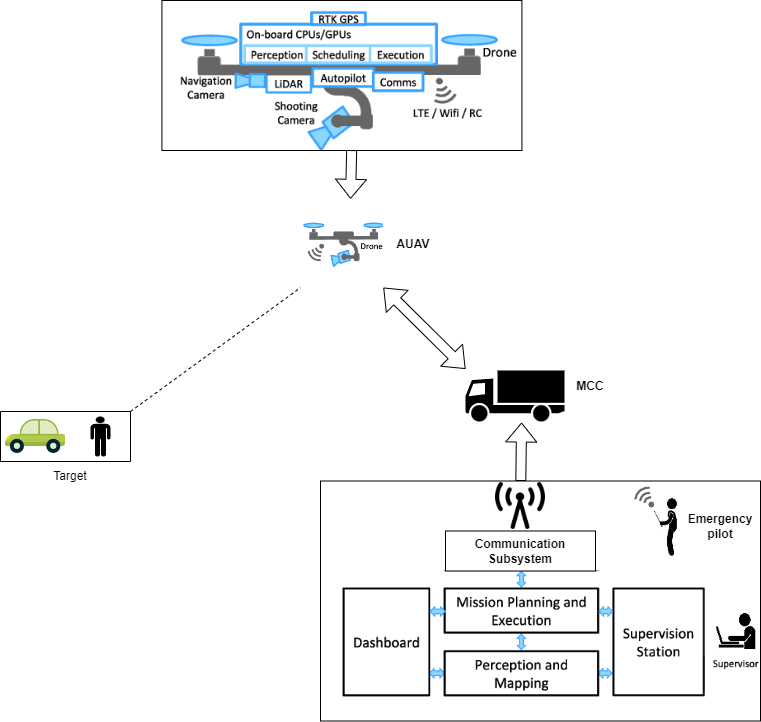
\includegraphics[scale=0.6]{CONOPS} 
   \end{center}

The AUAV will monitor and detect targets and is in constant communication with the MCC.

The AUAV has an AI-based decision-making capability with manual override and is capable of advanced (Signal/Image Processing) such as real-time Atmospheric Turbulence Compensation (ATC) and Automatic Target Recognition (ATR), which will produce the quickest real-time and highest spatial resolution images currently available.

The AUAV will be able to move in search-and-find maneuvers and track objects of interest (OoI).

Additionally, The AUAV is modular, allowing for easy modification and updating with the latest innovative hardware and software.

The system contain a Mobile Command Center (MCC) that can be placed indefinitely in inaccessible, remote places and will be fueled by a sound-proof, renewable energy source.In the event of an emergency, there will be a pilot who will assume control of the AUAV.

 \subsection{CONOP for UAV's Path Planning}
 \begin{center}
    Figure \ref{} below shows the concept of operations for UAV's pathplanning.
     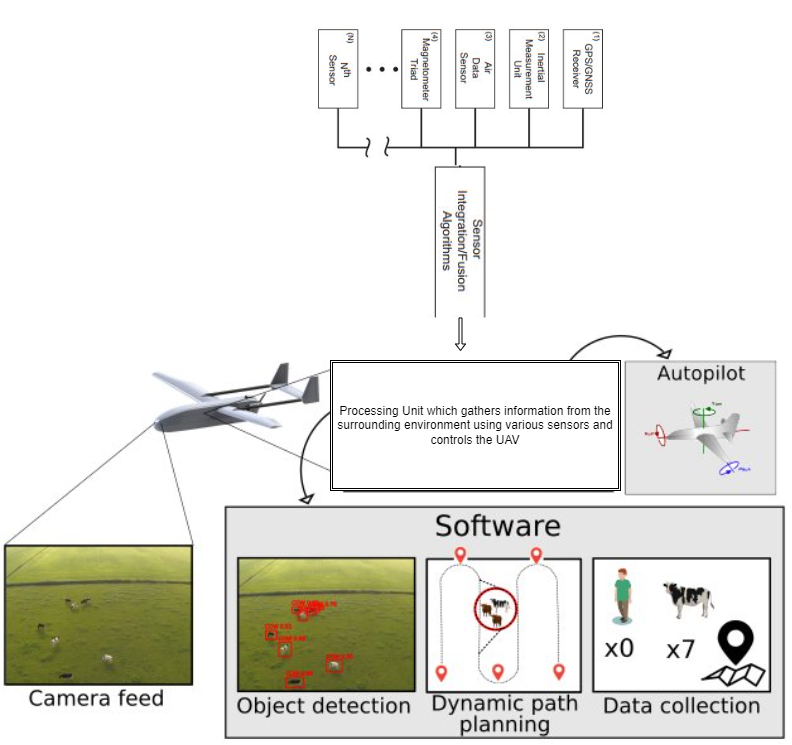
\includegraphics[scale=0.5]{ppCONOP}
 \end{center}
 With no connectivity to a base station, the AUAV system uses contemporary deep-learning techniques and hardware architectures to perform object recognition entirely onboard. In this manner, the UAV's maximum range is only constrained by its endurance.
 
 Additionally, we employ the identification of objects of interest to autonomously and effectively modify the UAV's flight path in order to capture additional photographs of those objects that might be valuable for further research in the future. 
 
 Given that the AUAV can be deployed in a variety of severe environments, its AI should be able to recognize and distinguish a relatively hostile environment.
 
 \subsubsection{Categorization of the Path Planning approaches}
 There are typically three ways that information about the environment where UAVs typically operate is available. The operational environment may be entirely known beforehand (for example, the geometry of barriers may be known), completely unknown, or only partially known (e.g., few portions are known, and some portions are explored and modeled during the flight.). Local Path Planning (LPP) and global Path Planning(GPP) are the two main categories for PP approaches based on the level of environmental knowledge. 
 
 In LPP, the surroundings is unknown, thus UAVs employ sensors or other tools to gather data about the surrounding area. In GPP, PP is carried out in a completely known environment, meaning that all environmental details are known beforehand.
 
 \begin{center}
    Figure \ref{} below shows the Categorization of the PP approaches based on the availability of information about operating environment.
     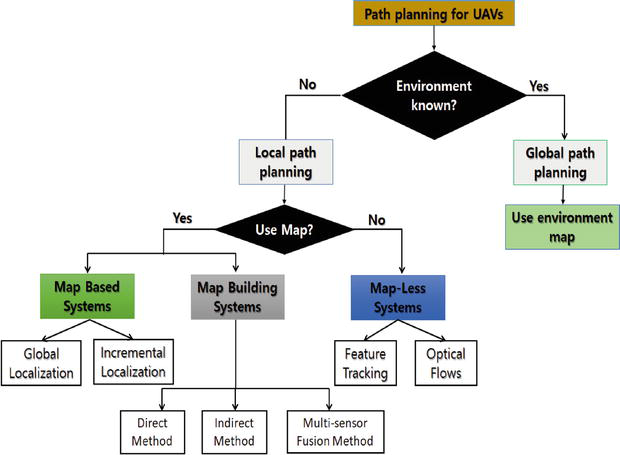
\includegraphics[scale=1.3]{pp block}
 \end{center}
 \hspace{1cm}
 \begin{center}
    Figure \ref{} displays the change in path of an AUAV
     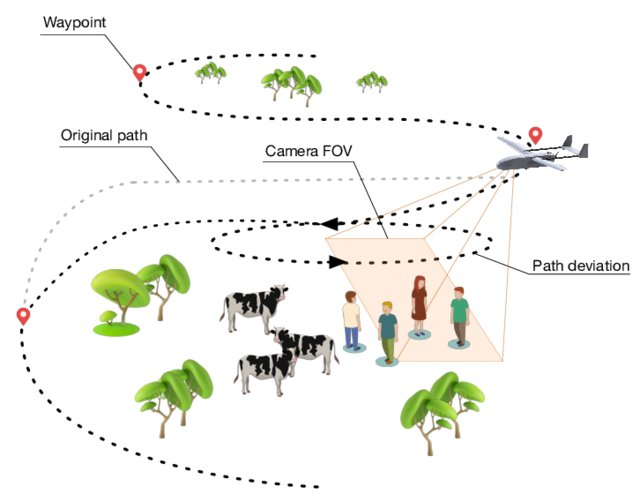
\includegraphics[scale=1.5]{PP}
    \end{center}
 The UAV will adjust its course after analyzing the data from its environment.
\end{fullwidth}

